\documentclass{standalone}
\usepackage{fkmath}
\usepackage{tikz}
\makeatletter
\tikzset{use path/.code=\tikz@addmode{\pgfsyssoftpath@setcurrentpath#1}}
\makeatother
\begin{document}
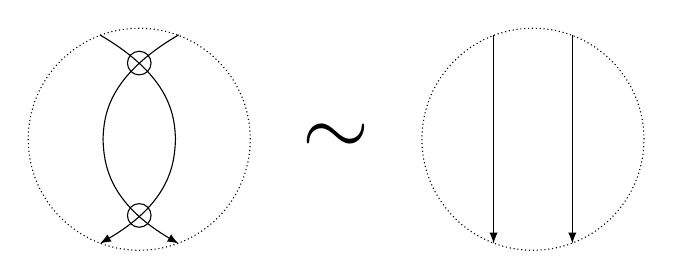
\begin{tikzpicture}[every node/.style={scale=1.25}]

  \def\defHalfReidII{

    \coordinate (p1) at (-.5, 1.325) {};
    \coordinate (p2) at (0.46, 0) {};
    \coordinate (p3) at (-.5, -1.325) {};

    \coordinate (c1) at (0.4, .8) {};
    \coordinate (c2) at (0.45, .3) {};
    \coordinate (c3) at (0.45, -.3) {};
    \coordinate (c4) at (.4, -.8) {};

    % \path (p1)
    \path[save path=\HalfR] (p1) .. controls (c1) and (c2) .. (p2) .. controls (c3) and (c4) .. (p3);
  }

  \pgfmathsetmacro{\bshift}{6}
  \pgfmathsetmacro{\cshift}{2*\bshift}
  \pgfmathsetmacro{\dshift}{3*\bshift}
  \pgfmathsetmacro{\bshiftcm}{\bshift cm}
  \pgfmathsetmacro{\cshiftcm}{\cshift cm}
  \pgfmathsetmacro{\dshiftcm}{\dshift cm}

  \begin{scope}
    \defHalfReidII

    \draw[-latex, use path=\HalfR];

    \begin{scope}[xscale=-1, yscale=1]
      \def\pointCols{\theNextPCol}
      \def\controlPointCols{\theNextCCol}
      \defHalfReidII

      % \draw[white, line width=7pt, use path=\HalfR];
      \draw[-latex, use path=\HalfR];
      \draw (0, .9675) circle (.15);
      \draw (0, -.9675) circle (.15);
    \end{scope}
    \draw[densely dotted] (0,0) circle (1.41);

  \end{scope}


  \begin{scope}[xshift=5cm]
    % \defHalfReidII
    \coordinate (p1) at (-.5, 1.325) {};
    \coordinate (p3) at (-.5, -1.325) {};

    \coordinate (q1) at (.5, 1.325) {};
    \coordinate (q3) at (.5, -1.325) {};

    % \draw[-latex, use path=\HalfR];
    \draw[-latex] (p1) -- (p3);
    \draw[-latex] (q1) -- (q3);

    \draw[densely dotted] (0,0) circle (1.41);

  \end{scope}

  \node () at (2.5, 0) {\Huge $\sim$};

\end{tikzpicture}
\end{document}
